\chapter{Software as a Service}

\section{Cloud Computing}
La differenza tra il possedere e l'utilizzare. E' questo l'aspetto cruciale del cambiamento apportato dal cloud computing rispetto al software tradizionale. Le risorse, che siano esse stesse archiviazione, elaborazione o qualsivoglia risorsa informatica, non sono mai ad hoc per un singolo utente, ma vengono assegnate on demand ai singoli utenti e appartengono ad un insieme condiviso da tutti gli altri utenti del prodotto utenti. Attraverso internet ogni utente può accedere a queste risorse in qualsiasi momento. Tali risorse vengono opportunamente allocate all'utente in maniera dinamica e completamente automatizzata. L'utente può utilizzare così anche software non installati sul proprio computer o usufruire di una memoria di massa accessibile da parte sua da qualsiasi dispositivo.
\paragraph{}
L'esperienza utente che si vuole fornire però è quella di un utilizzo esclusivo della risorsa, come nei software tradizionali, quando in realtà la risorsa viene solo sapientemente distribuita tra gli utenti. Ciò fa si che, potenzialmente, un singolo utente possa acquisire risorse notevolmente maggiori nel caso medio
\begin{figure}
	\centering
	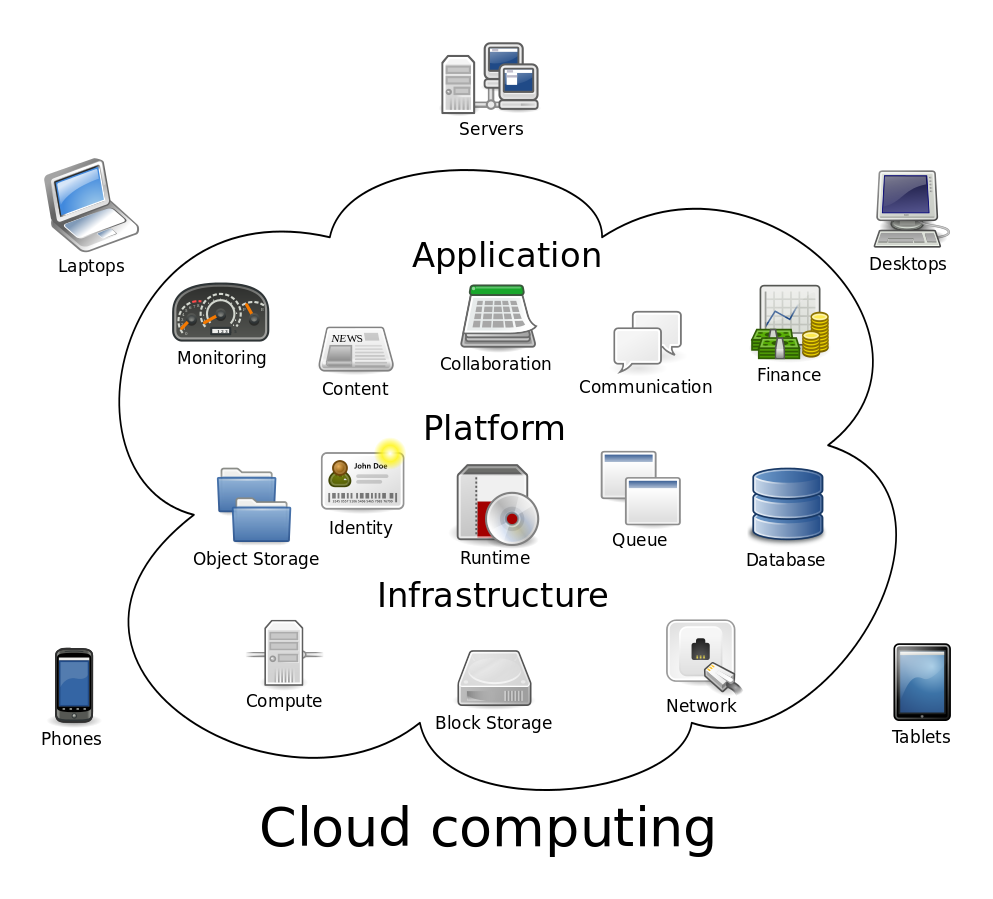
\includegraphics[width=0.7\linewidth]{capitoli/imgs/CloudComputing}
	\caption{Diagramma logico di una rete Cloud Computing}
	\label{fig:cloudcomputing}
\end{figure}
\subsection{Vantaggi del Cloud Computing}
\begin{itemize}
	\item Costo: \\
	Con l'avvento del cloud tutta la gestione dell'infrastruttura sottostante il software diviene a carico del provider. Vengono eliminate spese per la gestione dei data center locali. Facendo riferimento alla versione SaaS di BigFix ad esempio, il cliente viene sollevando dal pesante onere di utilizzare server locali e gestirne le relative connessioni. Il provider detiene tutto l'hardware di cui il cliente ha bisogno.
	
	\item Velocità: \\
	Anche quì ci risulta molto utile prendere ad esempio la suite di BigFix. quando un nuovo cliente acquista il prodotto nella sua versione on-premises, un'incaricato di IBM si reca presso il cliente e lì inizia un lungo processo di installazione della suite che può impiegare diverse ore. nella scenario SaaS il cambiamento è radicale. E' sufficente che il cliente compili una form online, dopo alcuni minuti poi riceve una mail con il link per accedere al servizio.
	
	\item Prestazioni \\
	La fornitura de servizi con questo paradigma consente di avere molta flessibilità nell'assegnazione delle risorse. Nel caso medio, l'ammontare delle risorse per il singolo utente è maggiore con l'utilizzo del cloud. Ciò ne consegue delle prestazioni molto maggiori.
	
	\item Affidabilità \\
	Operazioni di mirroring da parte dei provider dei servizi cloud fa sì che il backup dei dati sia continuo ed economico.
\end{itemize}

\section{Tipologie di servizi Cloud}
Il termine Cloud risulta in realtà molto generico. Esso comprende diverse tipologie di fornitura dei servizi, a seconda della risorsa che viene offerta dal provider. La maggior parte dei servizi di Cloud Computing rientrano in quattro tipologie principali, Infrastruttura distribuita come Servizio (IaaS, Infrastructure as a Service), Dati distribuiti come Servizio (DaaS, Data as a Service), Piattaforma distribuita come Servizio (PaaS, Platform as a Service) e Software come un Servizio (SaaS, Software as a Service). Andiamo a vedere nel dettaglio come, a seconda della tipologia di utilizzo del paradigma Cloud, queste tipoligie si differenziano.
\subsection{IaaS, Infrastructure as a Service}
E' la tipologia più basilare. Vengono messe a disposizione piattaforme di elaborazione. Utilizzando un IaaS si affittano le infrastrutture utili ai propri scopi, come add esempio server, macchine virtuali (VMs), risorse di archiviazione, reti e sistemi operativi. Può, inoltre, essere messo a isposizione anche hardware in remoto.
\subsection{DaaS, Data as a Service}
\subsection{PaaS, Platform as a Service}
\subsubsection{IBM Bluemix}
\subsection{SaaS, Software as a Service}

\section{Confronto tra SaaS e On Premise}
\paragraph{Vantaggi del Software On Premise}
\begin{itemize}
	\item  Controllo esclusivo su sistemi e dati
	\item Gestione interna dei dati sensibili
	\item Alto investimento iniziale ammortizzato nel lungo periodo
\end{itemize}

\paragraph{}
Il paradigma di fornitura on premise risulta ancora essere la soluzione più adatta nel caso in cui la gestione diretta dei dati sia fondamentale per policy aziendali oppure sia necessaria una maggiore flessibilità di configurazione per l’integrazione con altre architetture software. Un'altro requisito è che l'architettura fisica del software sia geograficamente localizzata.
